\documentclass[11pt]{utalcaDoc}
\usepackage{alltt}
\usepackage{underscore}
\usepackage[utf8]{inputenc}
\usepackage[activeacute,spanish]{babel}
\usepackage{verbatim}
\usepackage[pdftex]{graphicx}
\usepackage{epstopdf}
\usepackage{ae}
\usepackage{bigfoot}
\usepackage{enumerate}
\usepackage{amsmath}
\usepackage{amsfonts}
\usepackage{algorithm}
\usepackage{imakeidx}
\usepackage{algorithmic}
\usepackage{hyperref}



\title{{\bf Gestion de Redes}\\Laboratorio 5\\EIGRP}
\author{
    \bf{Profesor:} José Letelier (\texttt{jletelier@utalca.cl})\\ 
    \bf{Alumno Ayudante:} Erik Regla (\texttt{eregla09@alumnos.utalca.cl})\\ }
\date{\today}

\makeindex[columns=3, title=Alphabetical Index, intoc]
\begin{document}
\renewcommand{\figurename}{Figura~}
\renewcommand{\tablename}{Tabla~}

\maketitle
%\newpage
%\tableofcontents

%\newpage
\section{Descripción}
En este laboratorio se espera que el alumno se familiarize con los mecanismos de ruteo OSPF e EIGRP.

\section{Actividad a desarrollar}

A continuación se presenta una red consistente de tres enrutadores, de la cual se espera que se implemente RIP y posteriormente realice las siguientes actividades.

\begin{figure}[!ht]
  \centering
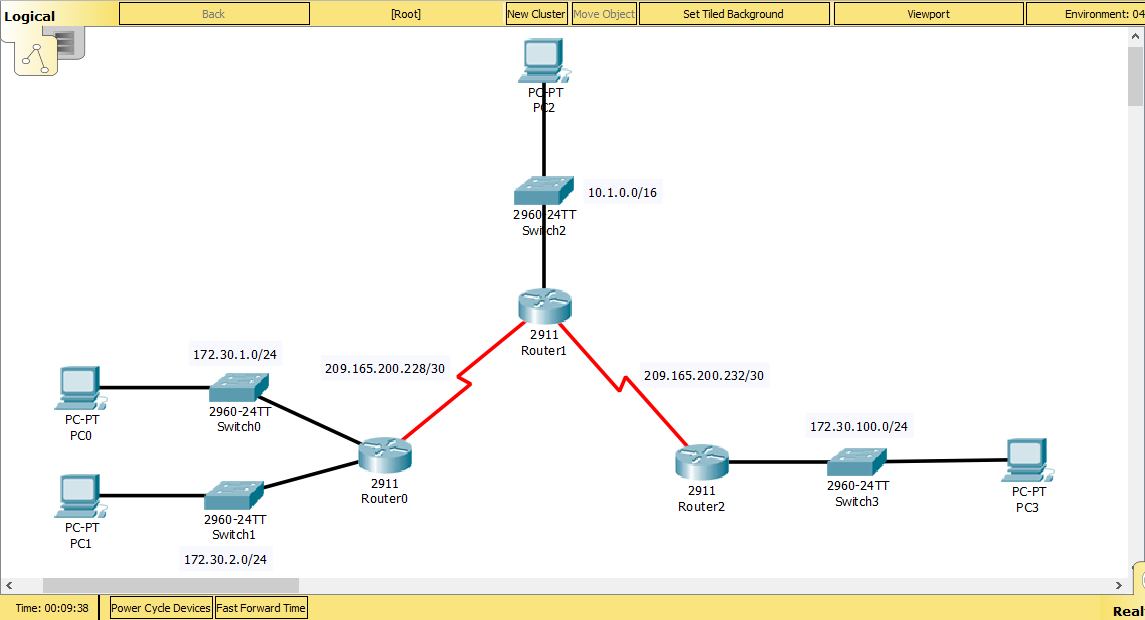
\includegraphics[scale=.3]{ipv4} 
  \caption{Diagrama IPv4}
  \label{FIGURE:1}
\end{figure}

\begin{figure}[!ht]
  \centering
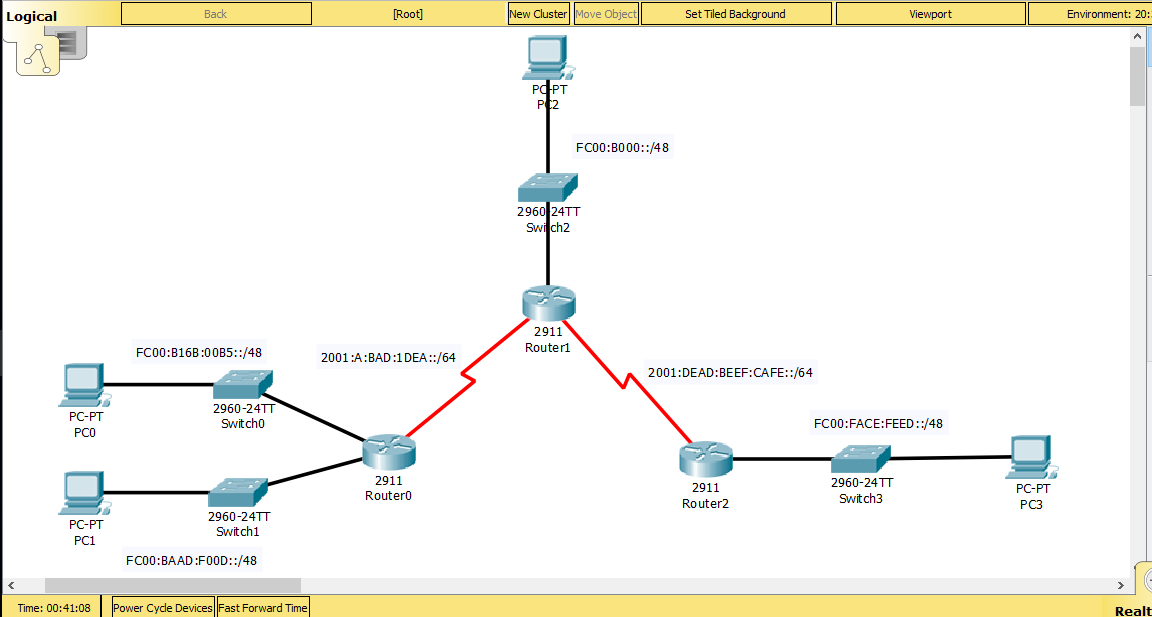
\includegraphics[scale=.3]{ipv6} 
  \caption{Diagrama IPv6}
  \label{FIGURE:2}
\end{figure}

\subsection{OSPF}
\begin{enumerate}
  \item {Implemente el diagrama de la Figura \ref{FIGURE:1}.}
  \item {Examine el estado de la red para cada uno de los tres enrutadores (utilize el comando \texttt{show ip interface brief}).}
  \item Examine las actualizaciones OSPF propagadas e indique las rutas actualmente establecidas.
  \item Agregue un enlace entre Router0 y Router2. Indique las rutas actualmente establecidas. ¿Sufrieron algún cambio?
  \item Cambie los costos de la ruta entre Router0 y Router1 sin desconectar las rutas. ¿Nota algún cambio en la red? Explique a que se deben sus observaciones.
  \item {Repita los pasos anteriores, implementando el diagrama de la Figura \ref{FIGURE:2}.}
\end{enumerate}

\subsection{EIGRP}
\begin{enumerate}
  \item {Implemente el diagrama de la Figura \ref{FIGURE:1}.}
  \item {Examine el estado de la red para cada uno de los tres enrutadores (utilize el comando \texttt{show ip interface brief}).}
  \item Examine las actualizaciones EIGRP propagadas e indique las rutas actualmente establecidas.
  \item Agregue un enlace entre Router0 y Router2. Indique las rutas actualmente establecidas. ¿Sufrieron algún cambio?
  \item {Repita los pasos anteriores, implementando el diagrama de la Figura \ref{FIGURE:2}.}
\end{enumerate}


\section{Evaluación}
\begin{itemize}
  \item{OSPF \textbf{3.0 pto}}
  \item{EIGRP \textbf{3.0 pto}}
\end{itemize}

\end{document}
